\subsection{Anexo A — Diagrama entidad-relación del modelo de datos}

El modelo relacional de ViaData — Medellín organiza el dominio de accidentalidad en tablas de hechos (\texttt{incidente}, \texttt{victima}), catálogos descriptivos (sexo, grupo de edad, condición, gravedad, clase de incidente), territorio (comuna, barrio) y tablas opcionales para infraestructura vial (\texttt{via}, \texttt{punto\_critico}), previstas en el esquema pero sin población desde Mede en la versión evaluada. La Figura~\ref{fig:esquema-bd} resume las relaciones principales; el DDL completo se incluye en el Anexo~B.

Las geometrías oficiales de comunas y barrios se gestionan en PostGIS (scripts \texttt{001}--\texttt{006} del pipeline de carga) y complementan las claves foráneas declarativas del registro Mede. El módulo de autenticación extiende \texttt{auth\_user} de Django mediante \texttt{perfil\_usuario} y la tabla \texttt{rol}.

\begin{figure}[H]
	\centering
	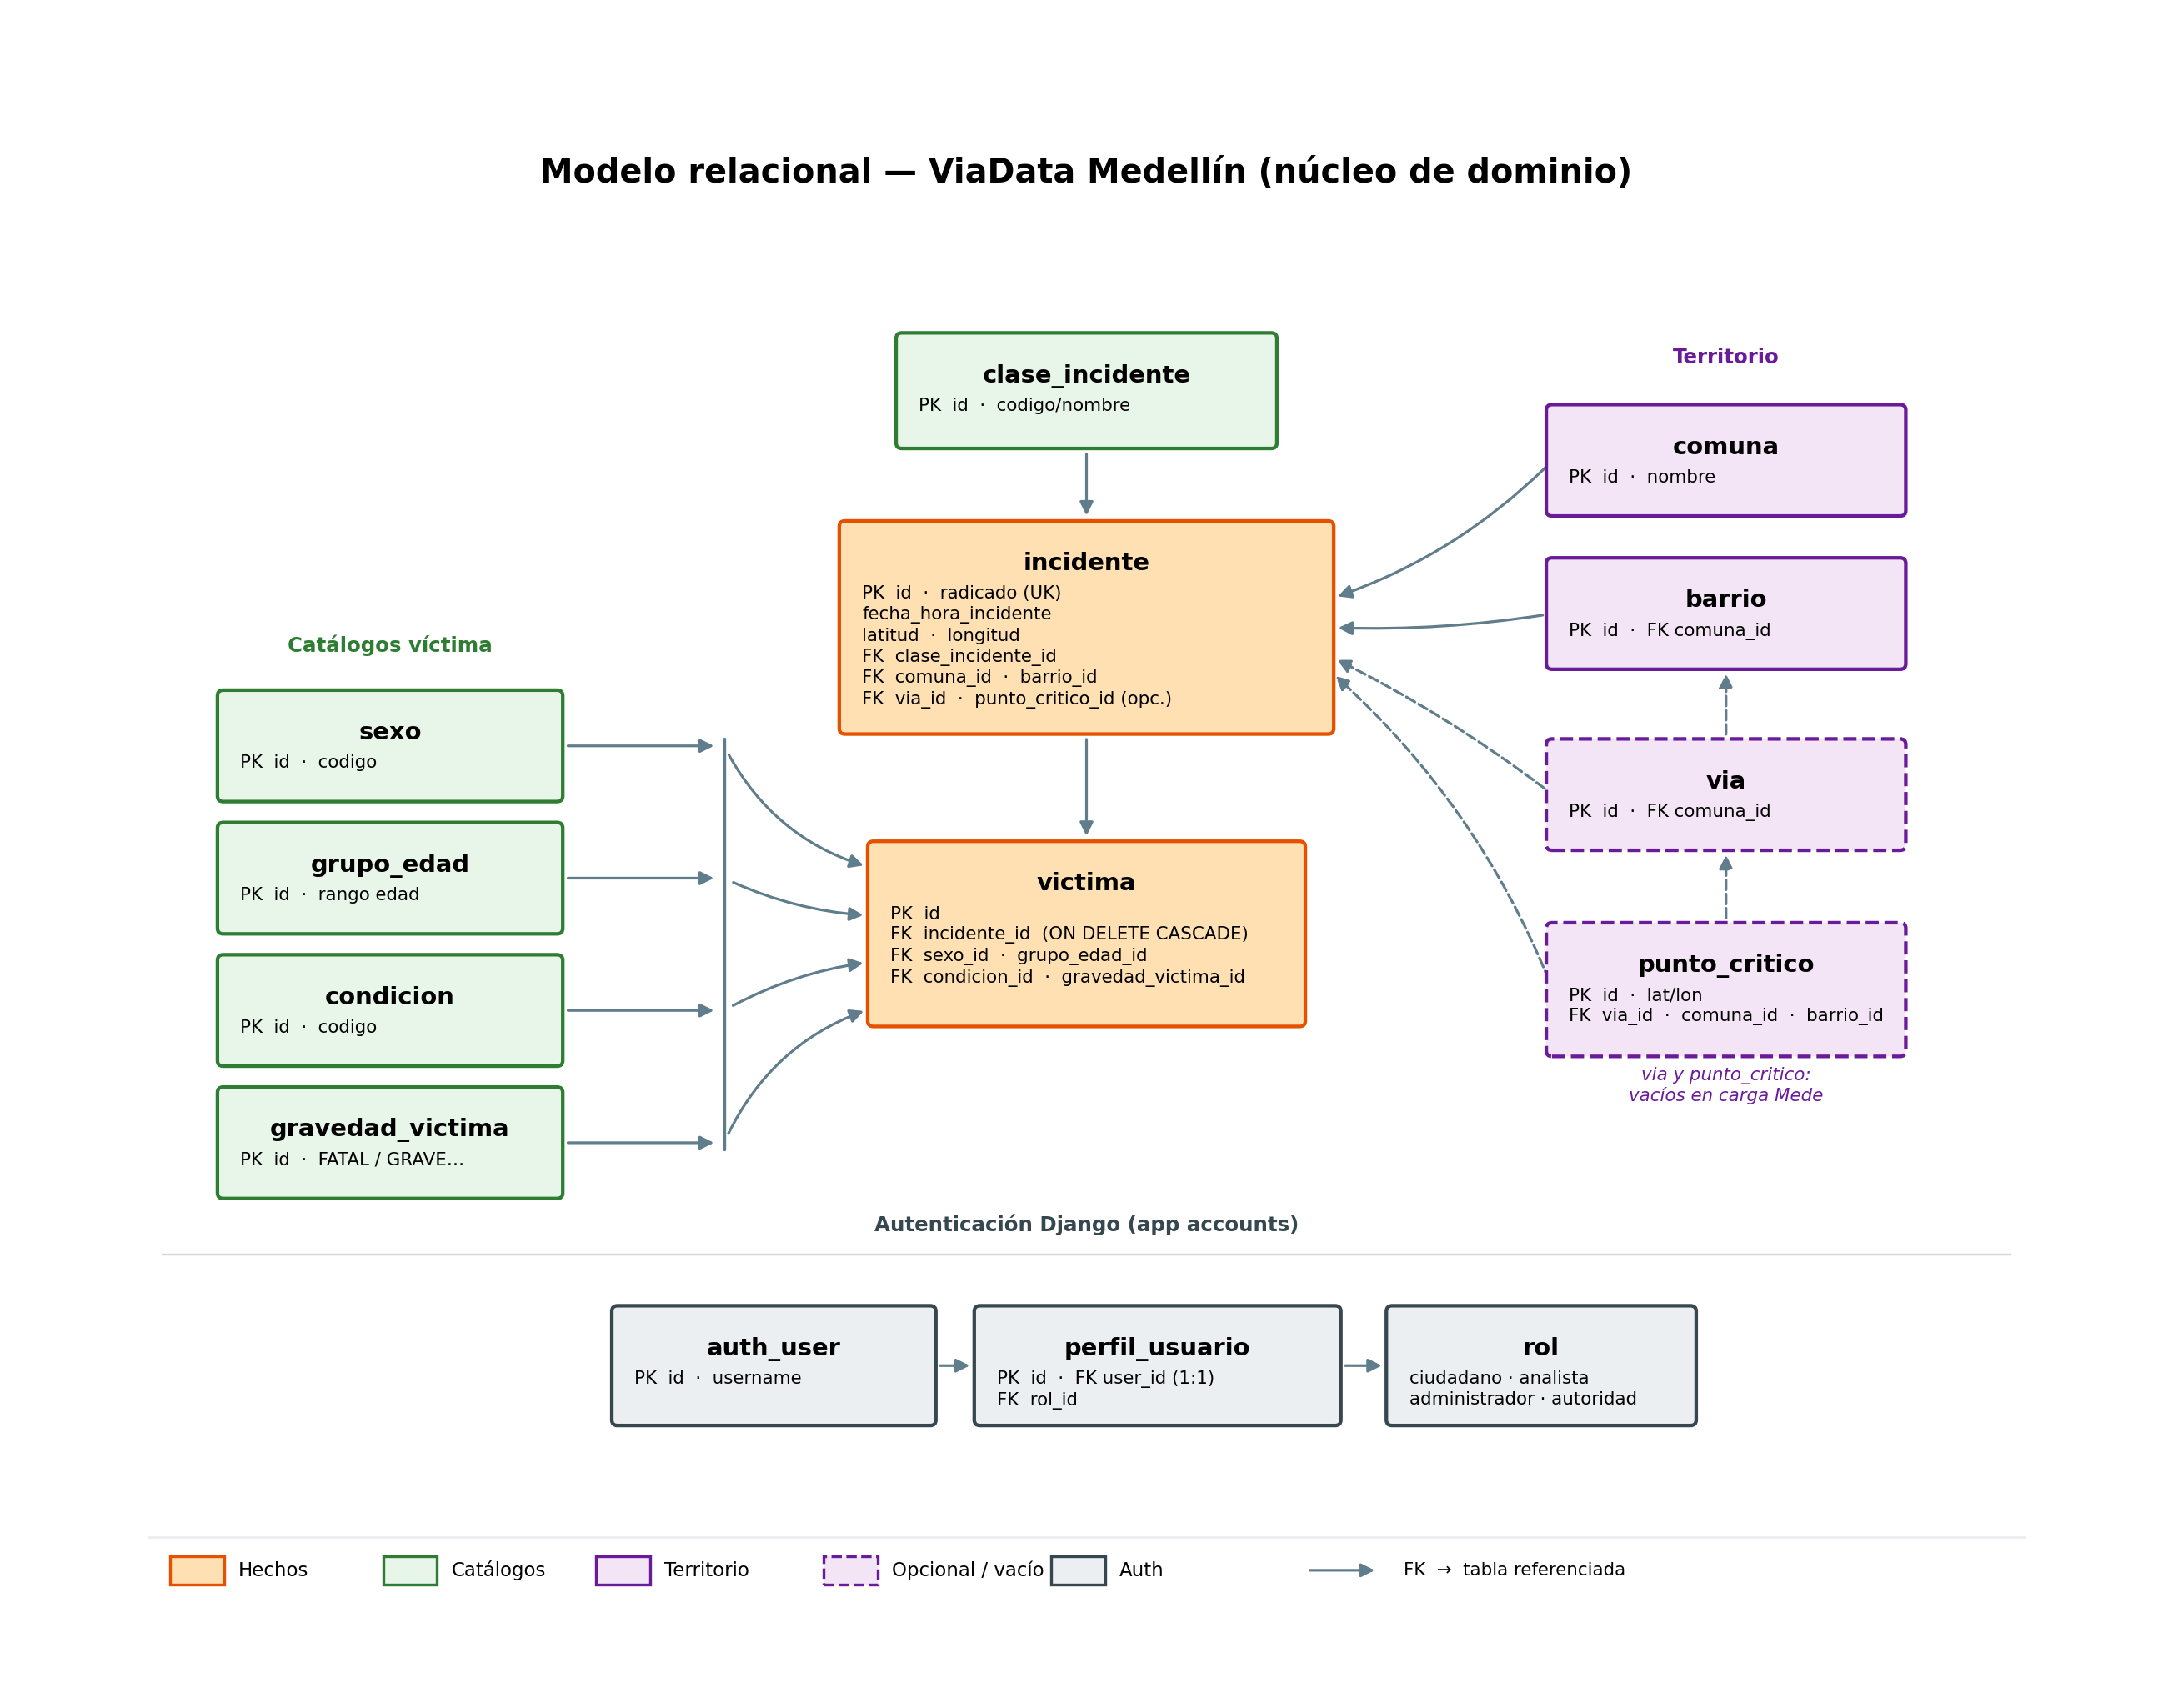
\includegraphics[width=0.98\linewidth]{images/fig_esquema_bd.png}
	\caption{Diagrama entidad-relación simplificado del núcleo de dominio}
	\label{fig:esquema-bd}
\end{figure}

\subsection{Anexo B — Esquema SQL de la base de datos}

El listado siguiente corresponde al archivo \texttt{Fuentes\_viaData/esquema\_base\_datos.sql}, que define catálogos, tablas principales, índices, vistas analíticas (\texttt{vista\_incidentes\_completa}, \texttt{vista\_estadisticas\_victimas}) y el bloque de autenticación Django (\texttt{auth\_user}, \texttt{perfil\_usuario}, \texttt{rol}, sesiones y permisos).

\begin{minted}[fontsize=\scriptsize,breaklines,breakanywhere]{sql}
-- Tablas principales (extracto)
CREATE TABLE incidente (
    id SERIAL PRIMARY KEY,
    radicado VARCHAR(50) UNIQUE NOT NULL,
    fecha_hora_incidente TIMESTAMP NOT NULL,
    clase_incidente_id INTEGER REFERENCES clase_incidente(id),
    latitud DECIMAL(10, 8),
    longitud DECIMAL(11, 8),
    comuna_id INTEGER REFERENCES comuna(id),
    barrio_id INTEGER REFERENCES barrio(id),
    via_id INTEGER REFERENCES via(id),
    punto_critico_id INTEGER REFERENCES punto_critico(id)
);

CREATE TABLE victima (
    id SERIAL PRIMARY KEY,
    incidente_id INTEGER NOT NULL REFERENCES incidente(id) ON DELETE CASCADE,
    sexo_id INTEGER REFERENCES sexo(id),
    grupo_edad_id INTEGER REFERENCES grupo_edad(id),
    condicion_id INTEGER REFERENCES condicion(id),
    gravedad_victima_id INTEGER REFERENCES gravedad_victima(id)
);
\end{minted}

El script íntegro incluye además datos semilla de catálogos, índices de consulta frecuente y comentarios de tablas de usuario. Se recomienda consultar el archivo fuente en el repositorio del proyecto para despliegues y migraciones.

\subsection{Anexo C — Manual de carga de datos (ETL Mede)}

La ingesta reproducible sigue el flujo documentado en \texttt{MANUAL\_CARGA\_DATOS\_BD.md}:

\begin{enumerate}
	\item Depuración del Excel con \texttt{mede\_limpieza.depurar\_mede()} (reglas únicas de calidad).
	\item Exportación a \texttt{Mede\_Victimas\_inci\_depurado.csv}.
	\item Carga idempotente con \texttt{carga\_mede\_pgadmin.sql}.
	\item Ejecución de scripts PostGIS y carga de polígonos (\texttt{cargar\_poligonos\_medellin}, \texttt{actualizar\_territorio\_espacial}).
	\item Verificación de conteos y del indicador G03 en la interfaz.
\end{enumerate}

Principio de diseño: toda regla de limpieza reside en \texttt{mede\_limpieza.py}; EDA, pipeline guiado y memoria de grado deben importar la misma lógica para garantizar reproducibilidad.

\subsection{Anexo D — Manual de instalación y ejecución}

Para replicar el entorno de desarrollo o demostración, \texttt{MANUAL\_INSTALACION\_EJECUCION.md} describe:

\begin{itemize}
	\item Requisitos: Python 3.11+, Node.js 20+, PostgreSQL 15+ con PostGIS, variables \texttt{.env} (base de datos, \texttt{GEMINI\_API\_KEY}).
	\item Backend: \texttt{python -m venv .venv}, \texttt{pip install -r requirements.txt}, \texttt{manage.py migrate}, \texttt{runserver :8000}.
	\item Frontend: \texttt{npm install}, \texttt{npm run dev} (puerto 5173).
	\item Pruebas: \texttt{python -m pytest -q} desde \texttt{backend/}.
	\item Usuario demo administrador: migración \texttt{0005\_seed\_admin\_user}.
\end{itemize}

\subsection{Anexo E — Evidencia numérica de predicciones}

Los resultados tabulados del módulo de predicciones se exportaron a CSV en \texttt{Fuentes\_viaData/}:

\begin{itemize}
	\item \texttt{predicciones\_seccion1\_proyeccion\_mensual.csv} (63 filas; 9 escenarios $\times$ 7 modelos).
	\item \texttt{predicciones\_seccion2\_prioridad\_territorial.csv}
	\item \texttt{predicciones\_seccion3\_carga\_territorial.csv}
	\item \texttt{predicciones\_seccion4\_proporcion\_fatales.csv}
	\item \texttt{predicciones\_seccion5\_patrones\_temporales.csv}
	\item \texttt{predicciones\_tres\_sigma\_evaluacion.csv}
	\item \texttt{MATRIZ\_ESCENARIOS\_CASO\_ESTUDIO.md} — caso de estudio escenario A (síntesis reproducible)
\end{itemize}

La metodología de evaluación y las decisiones adoptadas se documentan además en \texttt{EVALUACION\_MODULO\_PREDICCIONES.md} y en \texttt{VIADATA\_DOCUMENTACION\_INTEGRAL.md}.
